\documentclass[tikz,border=10pt]{standalone}
\usepackage{pgfplots}
\usepgfplotslibrary{groupplots}
\pgfplotsset{compat=1.18}

\begin{document}
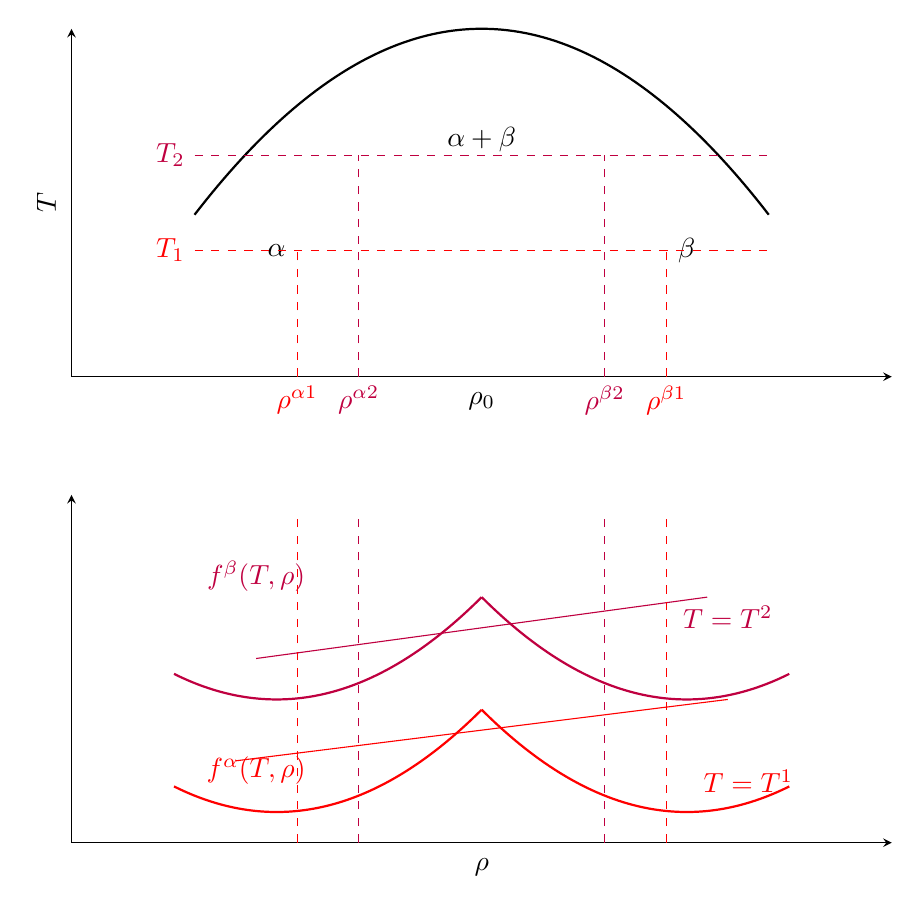
\begin{tikzpicture}
\begin{groupplot}[
    group style={group size=1 by 2, vertical sep=1.5cm},
    width=12cm,
    height=6cm,
    axis lines=left,
    xtick=\empty,
    ytick=\empty,
    xmin=0,
    xmax=4,
    clip=false
]

% Top panel: T vs rho_0
\nextgroupplot[
    xlabel={$\rho_0$},
    ylabel={$T$}
]
\addplot[thick,domain=0.6:3.4,samples=100] {2.2 - 0.6*(x-2)^2};
\addplot[black,domain=0.6:3.4,samples=100] {0};

% Region labels
\node at (axis cs:1.0,0.8) {$\alpha$};
\node at (axis cs:3.0,0.8) {$\beta$};
\node at (axis cs:2.0,1.5) {$\alpha+\beta$};

% T1 and T2 lines
\addplot[red,dashed] coordinates {(0.6,0.8) (3.4,0.8)};
\addplot[purple,dashed] coordinates {(0.6,1.4) (3.4,1.4)};
\node[red,left] at (axis cs:0.6,0.8) {$T_1$};
\node[purple,left] at (axis cs:0.6,1.4) {$T_2$};

% Mark densities on top axis
\addplot[red,dashed] coordinates {(1.1,0) (1.1,0.8)};
\addplot[red,dashed] coordinates {(2.9,0) (2.9,0.8)};
\addplot[purple,dashed] coordinates {(1.4,0) (1.4,1.4)};
\addplot[purple,dashed] coordinates {(2.6,0) (2.6,1.4)};

\node[red,below] at (axis cs:1.1,0) {$\rho^{\alpha 1}$};
\node[red,below] at (axis cs:2.9,0) {$\rho^{\beta 1}$};
\node[purple,below] at (axis cs:1.4,0) {$\rho^{\alpha 2}$};
\node[purple,below] at (axis cs:2.6,0) {$\rho^{\beta 2}$};

% Bottom panel: free energy curves vs rho
\nextgroupplot[
    xlabel={$\rho$},
    ylabel={},
    ymin=-0.2,
    ymax=3.2
]

% Curves for T1 (red)
\addplot[red,thick,domain=0.5:2.0,samples=100] {(x-1.0)^2+0.1};
\addplot[red,thick,domain=2.0:3.5,samples=100] {(x-3.0)^2+0.1};
\addplot[red] coordinates {(0.8,0.6) (3.2,1.2)};
\node[red] at (axis cs:3.3,0.4) {$T=T^1$};

% Curves for T2 (purple)
\addplot[purple,thick,domain=0.5:2.0,samples=100] {(x-1.0)^2+1.2};
\addplot[purple,thick,domain=2.0:3.5,samples=100] {(x-3.0)^2+1.2};
\addplot[purple] coordinates {(0.9,1.6) (3.1,2.2)};
\node[purple] at (axis cs:3.2,2.0) {$T=T^2$};

\node[purple] at (axis cs:0.9,2.4) {$f^\beta(T,\rho)$};
\node[red] at (axis cs:0.9,0.5) {$f^\alpha(T,\rho)$};

% Density markers aligned with top panel
\addplot[red,dashed] coordinates {(1.1,-0.2) (1.1,3.0)};
\addplot[red,dashed] coordinates {(2.9,-0.2) (2.9,3.0)};
\addplot[purple,dashed] coordinates {(1.4,-0.2) (1.4,3.0)};
\addplot[purple,dashed] coordinates {(2.6,-0.2) (2.6,3.0)};
\end{groupplot}
\end{tikzpicture}
\end{document}
